
%(BEGIN_QUESTION)
% Copyright 2010, Tony R. Kuphaldt, released under the Creative Commons Attribution License (v 1.0)
% This means you may do almost anything with this work of mine, so long as you give me proper credit

Part of this solar-heating control system uses a {\it dual-thermocouple} circuit to compare the temperature inside the solar collector against the temperature inside the house, preventing the circulation fan from running if the house is ever warmer than the collector:

$$\includegraphics[width=15.5cm]{i00377x01.eps}$$

Answer the following questions about this subsystem:

\begin{itemize}
\item{} Identify the thermocouple type used in this application, and determine whether or not this type is a good choice.
\vskip 10pt
\item{} Calculate the voltage measured at the input terminals of the transmitter, and also determine whether or not this transmitter needs to be enabled for reference junction compensation.
\vskip 10pt
\item{} Identify the meaning of the diamond-shaped PID symbol labeled ``TC''.
\end{itemize}

\underbar{file i00377}
%(END_QUESTION)





%(BEGIN_ANSWER)

These are type {\it T} thermocouples, sending 1.174 millivolts to the transmitter's input.  Cold junction compensation (CJC) should {\it not} be enabled in the transmitter, because we want to measure the difference in temperature between the collector and the house, not compensate for one of those thermocouples' voltages!

The diamond symbol is a {\it logic} device -- most likely a PLC -- used for on/off control of the fan.

%(END_ANSWER)





%(BEGIN_NOTES)

%INDEX% Measurement, temperature: thermocouple 
%INDEX% Process: solar hot-air collector control system

%(END_NOTES)

